% Uebung Parallelresonanzkreis mit Transformator  nach Brinkmeyer
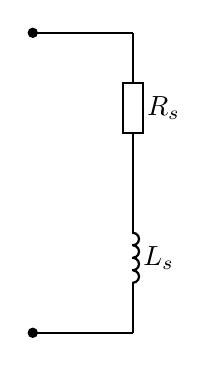
\begin{tikzpicture}[scale=2.54]%
% dpic version 2024.01.01 option -g for TikZ and PGF 1.01
\ifx\dpiclw\undefined\newdimen\dpiclw\fi
\global\def\dpicdraw{\draw[line width=\dpiclw]}
\global\def\dpicstop{;}
\dpiclw=0.8bp
\dpiclw=0.8bp
\dpicdraw[fill=black](0,0) circle (0.007874in)\dpicstop
\dpicdraw[fill=black](0,-1.5) circle (0.007874in)\dpicstop
\dpicdraw (0,0)
 --(0.5,0)\dpicstop
\dpicdraw (0.5,0)
 --(0.5,-0.25)\dpicstop
\dpicdraw (0.5,-0.5)
 --(0.55,-0.5)
 --(0.55,-0.25)
 --(0.45,-0.25)
 --(0.45,-0.5)
 --(0.5,-0.5)\dpicstop
\dpicdraw (0.5,-0.5)
 --(0.5,-0.75)\dpicstop
\draw (0.55,-0.375) node[right=-2bp]{$ R_s$};
\dpicdraw (0.5,-0.75)
 --(0.5,-1)\dpicstop
\dpicdraw (0.5,-1)
 --(0.494444,-1)\dpicstop
\dpicdraw (0.5,-1)
 ..controls (0.511165,-1) and (0.521481,-1.005956)
 ..(0.527063,-1.015625)
 ..controls (0.532646,-1.025294) and (0.532646,-1.037206)
 ..(0.527063,-1.046875)
 ..controls (0.521481,-1.056544) and (0.511165,-1.0625)
 ..(0.5,-1.0625)\dpicstop
\dpicdraw (0.5,-1.0625)
 --(0.494444,-1.0625)\dpicstop
\dpicdraw (0.5,-1.0625)
 ..controls (0.511165,-1.0625) and (0.521481,-1.068456)
 ..(0.527063,-1.078125)
 ..controls (0.532646,-1.087794) and (0.532646,-1.099706)
 ..(0.527063,-1.109375)
 ..controls (0.521481,-1.119044) and (0.511165,-1.125)
 ..(0.5,-1.125)\dpicstop
\dpicdraw (0.5,-1.125)
 --(0.494444,-1.125)\dpicstop
\dpicdraw (0.5,-1.125)
 ..controls (0.511165,-1.125) and (0.521481,-1.130956)
 ..(0.527063,-1.140625)
 ..controls (0.532646,-1.150294) and (0.532646,-1.162206)
 ..(0.527063,-1.171875)
 ..controls (0.521481,-1.181544) and (0.511165,-1.1875)
 ..(0.5,-1.1875)\dpicstop
\dpicdraw (0.5,-1.1875)
 --(0.494444,-1.1875)\dpicstop
\dpicdraw (0.5,-1.1875)
 ..controls (0.511165,-1.1875) and (0.521481,-1.193456)
 ..(0.527063,-1.203125)
 ..controls (0.532646,-1.212794) and (0.532646,-1.224706)
 ..(0.527063,-1.234375)
 ..controls (0.521481,-1.244044) and (0.511165,-1.25)
 ..(0.5,-1.25)\dpicstop
\dpicdraw (0.5,-1.25)
 --(0.494444,-1.25)\dpicstop
\dpicdraw (0.5,-1.25)
 --(0.5,-1.5)\dpicstop
\draw (0.53125,-1.125) node[right=-2bp]{$ L_s$};
\dpicdraw (0.5,-1.5)
 --(0,-1.5)\dpicstop
\end{tikzpicture}%
